\documentclass[aps,pra,showpacs,reprint,onecolumn,notitlepage]{revtex4-1}

\usepackage{siunitx}
\sisetup{separate-uncertainty}
\usepackage{graphicx}
\usepackage{dcolumn}
\usepackage{bm}
\usepackage{hyperref}
\usepackage{epstopdf}% To incorporate .eps illustrations using PDFLaTeX, etc.
%\usepackage{subfigure}% Support for small, `sub' figures and tables
\usepackage{placeins}
\usepackage{color}
\usepackage{mathtools}

%math
\usepackage{amssymb}
\usepackage{amsmath} %right equation numbering + mathenvironments
\usepackage{bm} 
\renewcommand{\baselinestretch}{1.1}
\usepackage{xfrac} %%\sfrac for 1/2 type fractions

  %OWN COMMANDS
\newcommand{\enquoteit}[1]{``#1''}
\newcommand{\avr}[1]{\mathop{\left\langle #1 \right\rangle}\nolimits}
\newcommand{\create}[0]{\mathop{\hat{a}^{\dagger}}\nolimits}
\newcommand{\anihil}[0]{\mathop{\hat{a}^{}}\nolimits}
\newcommand{\bra}[1]{\mathop{\left\langle #1 \right|}\nolimits}
\newcommand{\ket}[1]{\mathop{\left| #1 \right\rangle}\nolimits}
\newcommand{\tx}[1]{\textnormal{#1}}
\def\@fnsymbol#1{\ensuremath{\ifcase#1\or *\or \dagger\or \ddagger\or
   \mathsection\or \mathparagraph\or \|\or **\or \dagger\dagger
   \or \ddagger\ddagger \else\@ctrerr\fi}}
\newcommand{\ssym}[1]{^{\@fnsymbol{#1}}}

\begin{document}

\title{Controlling the spectrum of single photons from\\ triply-resonant parametric down-conversion}
\pdfoutput=1
\author{author et al.$^{1,2,*}$}
%\author{Gerhard Schunk$^{1,2,3,*}$}
%\author{Ulrich Vogl$^{1,2}$}
%\author{Florian Sedlmeir$^{1,2,3}$}
%\author{Dmitry V. Strekalov$^{1,2}$}
%\author{Alexander Otterpohl$^{1,2}$}
%\author{Valentin Averchenko$^{1,2,3}$}
%\author{Harald G. L. Schwefel$^{1,2,4}$}
%\author{Gerd Leuchs$^{1,2}$}
%\author{Christoph Marquardt$^{1,2,6}$}
\affiliation{$^{1}$Max Planck Institute for the Science of Light, G\"{u}nther-Scharowsky-Stra\ss e 1/Building 24, 90158 Erlangen, Germany}              
\affiliation{$^{2}$Institute for Optics, Information and Photonics, University Erlangen-N\"{u}rnberg, Staudtstr.7/B2, 90158 Erlangen, Germany}
\affiliation{$^{3}$SAOT, School in Advanced Optical Technologies, Paul-Gordan-Str. 6, 91052 Erlangen, Germany}
%\affiliation{$^{4}$Department of Physics, University of Otago, 730 Cumberland Street, Dunedin 9016, New Zealand}
%\affiliation{$^{5}$Department of Physics, Technical University of Denmark, Fysikvej Building 309, 2800 Lyngby, Denmark}
%\affiliation{$^{*}$Corresponding author: Gerhard.Schunk@mpl.mpg.de}

%%%%%%%%%%%%%%%%%%%%%%%%%%%%%%%%%%%%%%%%%%%%%%%%%%%%%%

\begin{abstract}
* goal: efficienct single photon atom interaction \\
* insdistinguishable photon pairs widely studied for non-resonant systems. \\
* We show how PDC phase-matching temperature affects the photon spectra.
\end{abstract}

\maketitle 

%\tableofcontents

\section{Introduction}

\section{Spectrum of the parametric photons depending frequency mismatch}
The optical resonator coupling can be described by the resonator bandwidth $\gamma\,$:
\begin{align}
	\gamma_\textrm{} = \gamma^{\prime}_\textrm{} + \gamma^{\prime\prime}_\textrm{} \, .
	\label{eq:resbandwidth}
\end{align}

The resonator bandwidth is the sum of the external coupling rate $\gamma^{\prime}_\textrm{}$ and the internal loss rate $\gamma^{\prime\prime}_\textrm{}$ and can be interpreted as an overall intensity decay rate of the internal resonator field. This interpretation becomes obvious in ring down spectroscopy, where a switch-off of the external pump at time $t=0$ leads to an exponential decay of the internal field given by $|\alpha(t)|^2 = |\alpha(t=0)|^2 \cdot \tx{e}^{- 2 \pi \gamma t}\,$. The coupling rates $\gamma^\prime$ and $\gamma^{\prime\prime}$ are directly connected to the mirror transmittance $T$ and the material absorption $b\,$ \cite{Bachor2004}:

The resonator frequency response is then given by
\begin{align}
	\mathcal{G} (\nu) = 1 / \left( 1 - i 2 {\left[ \frac{\nu-\nu_0}{\gamma} \right]}  \right) = \frac{1}{ {1 - i 2 \delta} } \,.
	\label{eq:cavityresponse}
\end{align}

The Hamiltonian $\hat{H}$ for the three interacting fields is:
\begin{align}
	\hat{H} = {\sum_{j \in \left\lbrace \tx{p,s,i} \right\rbrace}{\hslash 2 \pi \, \nu (\ell_\textrm{j},\textrm{q}_\textrm{j},\textrm{p}_\textrm{j}) \left( \hat{a}\ssym{2}_\tx{j} \hat{a}_\tx{j} + \sfrac{1}{2} \right)} }
	+ \underbrace{i \hslash \pi  \left( {g} \hat{a}_\tx{p}  \hat{a}_\tx{s}\ssym{2} \hat{a}_\tx{i}\ssym{2} - \tx{h.c.} \right) }_{ \equiv \hat{H}_\tx{I}} \,.
	\label{eq:HamiltonianPDC}
\end{align}

In the following, we consider the case of a monochromatic pump at frequency $\nu_\tx{p}$.  The parametric spectum can be calculated by solving the coupled wave equations. The different frequency components of signal and idler are conveniently summarized by the frequency mismatch $\Delta$, which is the residual mismatch between the pump electric field at frequency $\nu_\textrm{p}$ and the parametric resonance frequencies $\nu (\ell_\textrm{s,i},\textrm{q}_\textrm{s,i},\textrm{p}_\textrm{s,i})$ normalized to the average bandwidth $\gamma_\tx{si}$ of signal and idler:
\begin{align}
 	\Delta = \underbrace{\frac{2}{\gamma_\textrm{s}+\gamma_\textrm{i}} }_{ = 1 / \gamma_\tx{si}} \cdot \left[ \nu_\textrm{p} - \nu (\ell_\textrm{s},\textrm{q}_\textrm{s},	\textrm{p}_\textrm{s} ) - \nu (\ell_\textrm{i},\textrm{q}_\textrm{i},\textrm{p}_\textrm{i} ) \right] \,.
 	\label{eq:SPDCfrequ}
\end{align} 

For $\Delta=0$, energy conservation allows for a maximally efficient conversion from the pump electric field frequency $\nu_\textrm{p}$ to the exact parametric resonance frequencies $\nu (\ell_\textrm{s,i},\textrm{q}_\textrm{s,i},\textrm{p}_\textrm{s,i})$. In a typical experiment, the pump laser at frequency $\nu_\textrm{p}$ is locked to the resonance frequency of the pump mode ($\delta_\textrm{p}=0$) for a high intracavity power. The frequency mismatch $\Delta$ is then controlled via the temperature-dependence of the resonance frequencies $\nu (\ell_\textrm{p,s,i},\textrm{q}_\textrm{p,s,i},\textrm{p}_\textrm{p,s,i})$.
\begin{figure}[htb]
	\centering
	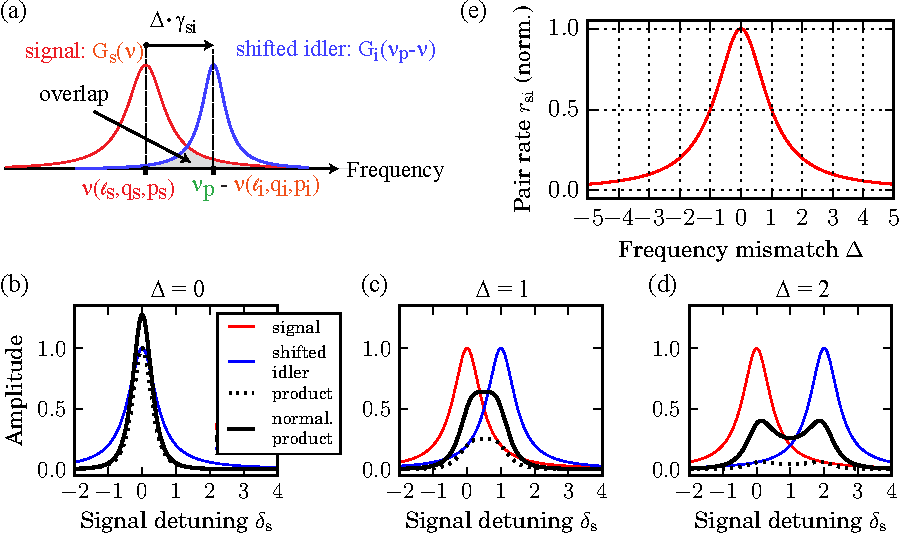
\includegraphics[scale=0.9]{pictures/teo_SPDC_spectrum/SPDC_spectrum_1.pdf}
	\caption{Frequency spectrum of parametric down-conversion below threshold. (a) The overlap integral of the parametric response functions $\tx{G}_\tx{s,i}(\nu) = |\mathcal{G}_\tx{s,i}(\nu)|^2$ in frequency space (see Eq.~\ref{eq:cavityresponse_c}) determines the parametric photon numbers $N_\tx{s,i}$ according to Eq.~\ref{eq:twophotonstate}. (b-d) The product of the signal $\tx{G}_\tx{s}(\nu)$ and the shifted idler $\tx{G}_\tx{i}(\gamma_\tx{si}\Delta + \nu (\ell_\textrm{s},\textrm{q}_\textrm{s},\textrm{p}_\textrm{s} ) +\nu (\ell_\textrm{i},\textrm{q}_\textrm{i},\textrm{p}_\textrm{i} ) -\nu) = \tx{G}_\tx{i}(\nu_\tx{p}-\nu)$ response functions ($\gamma_\tx{s}=\gamma_\tx{i} = \gamma_\tx{si}$ in this example) are plotted for various frequency mismatches $\Delta$ (see Eq.~\ref{eq:SPDCfrequ}). The black line shows the product normalized to a unity area. (e) The pair production rate ${r_\tx{si} \propto \left( 1+\Delta^2 \right)^{-1}}$ (see Eq.~\ref{eq:rategenbelow}) as a function on the frequency mismatch $\Delta$  is Lorentzian.} 
	\label{fig:spdc_spectrum}
\end{figure}

The oscillation threshold for the optical pump power $P^\tx{}_\textrm{th}\left( \delta_\textrm{p},\Delta\right)$ is then given by
\begin{align}
	 P_\textrm{th} \left( \delta_\textrm{p},\Delta\right) = \hslash 2 \pi \nu_\tx{p}  |\alpha^\tx{in}_\tx{p}|^2 = P_\textrm{0} \cdot \left(1 + 4 \delta_\textrm{p}^2 \right) \cdot \left(1 +  \Delta^2\right)   \,.
\label{eq:threshold}
\end{align}

In the limit of low gain, i.e far below threshold, we can iteratively solve the coupled wave equation for pump, signal, and idler with first-order pertubation theory for $|\alpha_\tx{p} g| / \gamma_\tx{s,i} \ll 1$. The noise power $S_\tx{s,i} (\nu)$ of the parametric photons at frequency $\nu$ in the resonator follows from 
\begin{alignat}{3}
	\avr{\hat{a}_\tx{s,i}\ssym{2} \left( \nu^\prime \right)\cdot \hat{a}_\tx{s,i} \left( \nu \right) } &= S_\tx{s,i} (\nu)  \cdot \delta(\nu - \nu^\prime) 
	\notag \\ 
	&=  \frac{2}{\pi \gamma_\tx{s,i}} \frac{ \tx{N}_\tx{p} }{\tx{N}_\tx{th}}  {{G}_\tx{s,i}\left( \nu + \nu (\ell_\textrm{s,i},\textrm{q}_\textrm{s,i},\textrm{p}_\textrm{s,i} ) \right)} \, {{G}_\tx{i,s} \left( \gamma_\tx{si} \Delta + \nu (\ell_\textrm{i,s},\textrm{q}_\textrm{i,s},\textrm{p}_\textrm{i,s} )  - \nu \right)}  \, .
\label{eq:spectrum}
\end{alignat} 

Vacuum fluctuations\footnote{For an evaluation of Eq.~\ref{eq:spectrum}, only the term $\avr{ \hat{\tx{f}}_\tx{s,i} \left( \nu\right) \hat{\tx{f}}_\tx{s,i} \ssym{2} \left( \nu\right) } = 2 \pi \gamma_\tx{s,i}$ gives a non-zero contribution according to Eq.~\ref{eq:commutator},~\ref{eq:inputoutput},~and~\ref{eq:rateequationslong}.} $\hat{\tx{f}}_\tx{i} \left( \nu\right)$ of the idler mode drive the signal noise power, and visa verse. By integrating over the full frequency space (see Fig.~\ref{fig:SPDCmodesill_shifted}), we get the number $N_\tx{s,i}$ of signal and idler photons in the resonator: 
\begin{align}
	N_\tx{s,i} &= \int S_\tx{s,i} (\nu) \, \tx{d} \nu = \frac{1}{\gamma_\tx{s,i}} \frac{ \tx{N}_\tx{p} }{\tx{N}_\tx{th}}  \frac{\gamma_\tx{s} \gamma_\tx{i} }{\gamma_\tx{si}} \frac{1}{1 + \Delta^2} \,  .  
	\label{eq:twophotonstate}
\end{align}

In parametric down-conversion, signal and idler are produced in pairs. Hence, we can define the rate of photon pair production ${r_\textrm{si}}{}$ in the resonator:
\begin{align}
	{r_\textrm{si}}{} = 2 \pi \,  \frac{\gamma^{}_\textrm{s} \gamma^{}_\textrm{i}}{\gamma^{}_\textrm{s} + \gamma^{}_\textrm{i}}  \frac{P^\tx{in}_\textrm{p}}{P_\textrm{th}\left( \delta_\textrm{p},\Delta \right)}  \, ,\quad (P^\tx{in}_\textrm{p} \ll P_\textrm{th})  \,.
\label{eq:rategenbelow}
\end{align}

The simultaneous generation of signal and idler  favors a description of parametric down-conversion in terms of temporal correlation functions \cite{Fekete2013,glauber1963,Michael2013,Ou1999,Scholz2009,Bocquillon2009,Bettelli2010,Luo2015}. The time-dependent annihilation and creation operators stem from the Fourier back-transformation $\int \tx{d} \nu \, \hat{a}(\nu) \, \tx{e}^{i2 \pi \nu t} \rightarrow \hat{a}(t)$ of Eq.~\ref{eq:rateequationsshortfour} and the input-output relation given by Eq.~\ref{eq:inputoutput}. The normalized cross-correlation function $\tx{g}^{(2)}_\textrm{si}(\tau)$  between signal and idler in terms of the detection time difference $\tau = t_\tx{s} - t_\tx{i}$ is given by
\begin{align}
	\tx{g}^{(2)}_\textrm{si}(\tau) &= \frac{ \avr{\hat{a}_\tx{s}^{\dagger \tx{out}} \left(t\right) \hat{a}_\tx{i}^{\dagger \tx{out}}\left(t+\tau\right) \hat{a}^{\tx{out}}_\tx{s} \left(t\right) \hat{a}^{\tx{out}}_\tx{s}\left(t+\tau\right)} }{\avr{\hat{a}^{\dagger \tx{out}}_\tx{s} \left(t\right) \hat{a}^{\tx{out}}_\tx{s} \left(t\right)} \avr{ \hat{a}^{\tx{out}}_\tx{i} \left(t\right) \hat{a}^{\dagger \tx{out}}_\tx{i}\left(t\right)} }  \notag \\
	&= 1 + \frac{ P_\textrm{th}\left( \delta_\textrm{p},\Delta \right) }{ P^\tx{in}_\textrm{p}  }  \cdot 
	\begin{cases}
        \tx{exp} \left(   2 \pi \gamma_\tx{i} \tau \right)  &\tx{for } \tau < 0  \\
        \tx{exp} \left( - 2 \pi \gamma_\tx{s} \tau \right) &\tx{for } \tau  > 0
        \end{cases}  \, .
	\label{eq:crosscorrelation}
\end{align}

The cross-correlation is usually measured by direct detection of signal and idler.

\section{Parametric down-conversion depending on the phase-matching temperature}

\section{Locking the phase-matching temperature}

\section{References}
	\bibliographystyle{apsrev4-1}
	\bibliography{MyCollection}
%	

%\begin{thebibliography}{10}
%
%\newcommand{\enquote}[1]{``#1''}
%\bibitem{Specht2011}
%H.~P. Specht, C.~N\"{o}lleke, A.~Reiserer, M.~Uphoff, E.~Figueroa, S.~Ritter
%  and G.~Rempe.
%\newblock \emph{{A single-atom quantum memory}}.
%\newblock Nature \textbf{473}, 190 (2011).
%\end{thebibliography}

\end{document}

